\documentclass[11pt]{article}

% ---------- geometry ----------
\usepackage[letterpaper,top=0.9in,bottom=0.9in,left=1in,right=1in]{geometry}

% ---------- fonts ----------
\usepackage[T1]{fontenc}
\usepackage{charter}
\usepackage[scaled=0.92]{helvet}
\usepackage{microtype}

% ---------- no hyphenation anywhere ----------
\usepackage[none]{hyphenat}
\hyphenpenalty=10000
\exhyphenpenalty=10000
\tolerance=2000
\emergencystretch=4em

% ---------- color: black, gray, white ----------
\usepackage{xcolor}
\definecolor{ink}{gray}{0.13}
\definecolor{mid}{gray}{0.42}
\definecolor{soft}{gray}{0.58}
\definecolor{rulegray}{gray}{0.80}
\definecolor{fillgray}{gray}{0.90}
\definecolor{barlite}{gray}{0.78}
\definecolor{barmid}{gray}{0.52}
\definecolor{bardark}{gray}{0.17}
\definecolor{zecgold}{RGB}{224,160,32}
\definecolor{goldtint}{RGB}{250,243,228}
\color{ink}

% ---------- spacing ----------
\usepackage{parskip}
\setlength{\parskip}{0.5\baselineskip}
\usepackage{setspace}
\setstretch{1.06}

% ---------- headings with a divider rule ----------
\usepackage{titlesec}
\titleformat{\section}{\sffamily\large\bfseries\color{ink}}{\thesection}{0.7em}{}[\vspace{2.5pt}{\color{zecgold}\titlerule[0.9pt]}]
\titlespacing*{\section}{0pt}{1.1\baselineskip}{0.45\baselineskip}
\titleformat{\subsection}{\sffamily\normalsize\bfseries\color{ink}}{\thesubsection}{0.6em}{}
\titlespacing*{\subsection}{0pt}{0.8\baselineskip}{0.2\baselineskip}

% ---------- tables, lists ----------
\usepackage{booktabs}
\usepackage{array}
\usepackage{enumitem}
\setlist[itemize]{leftmargin=1.3em,itemsep=3pt,topsep=2pt,parsep=0pt}
\renewcommand{\arraystretch}{1.25}

% ---------- running header ----------
\usepackage{fancyhdr}
\pagestyle{fancy}
\fancyhf{}
\newcommand{\hdot}{\hspace{0.5em}{\color{zecgold}\textperiodcentered}\hspace{0.5em}}
\fancyhead[L]{\footnotesize\sffamily\color{soft}UBC 2026\hdot Purdue University}
\fancyhead[R]{\footnotesize\sffamily\color{soft}Zcash (ZEC) Short\hdot Track 03}
\fancyfoot[C]{\footnotesize\sffamily\color{soft}\thepage}
\renewcommand{\headrule}{\color{rulegray}\hrule height 0.4pt\vspace{2pt}}
\renewcommand{\footrulewidth}{0pt}

% ---------- charts ----------
\usepackage{pgfplots}
\pgfplotsset{compat=1.18}
\usetikzlibrary{positioning}

% ---------- design helpers ----------
\newcommand{\figtitle}[1]{\par\vspace{2pt}{\sffamily\bfseries\small\color{ink} #1}\par\vspace{1pt}}
\newcommand{\figcap}[2]{\par\vspace{3pt}{\footnotesize\sffamily\color{mid}\textbf{#1}\quad #2}\par}
\newcommand{\exlabel}[1]{{\sffamily\bfseries\footnotesize\color{ink} #1}\par\vspace{2pt}}
\newcommand{\excap}[1]{\par\vspace{1pt}{\scriptsize\sffamily\color{mid} #1}\par}
\newcommand{\statcell}[2]{\begin{minipage}[t]{0.235\linewidth}\centering{\sffamily\bfseries\fontsize{18}{20}\selectfont #1}\\[3pt]{\scriptsize\sffamily\color{mid}\MakeUppercase{#2}}\end{minipage}}
\newcommand{\statband}[1]{\par\vspace{6pt}{\color{zecgold}\hrule height 0.9pt}\vspace{8pt}\noindent #1 \par\vspace{8pt}{\color{zecgold}\hrule height 0.9pt}\par\vspace{3pt}}
\newcommand{\pullquote}[2]{\par\vspace{7pt}\begin{center}\begin{minipage}{0.9\linewidth}\centering{\fontsize{13}{16}\selectfont\color{ink}\itshape #1}\\[4pt]{\footnotesize\sffamily\color{mid}\MakeUppercase{#2}}\end{minipage}\end{center}\vspace{4pt}}

\begin{document}

% ======================= TITLE PAGE =======================
\thispagestyle{empty}
\vspace*{1.05in}

{\sffamily\footnotesize\color{soft}\MakeUppercase{Franklin Crypto Research Competition}\\[3pt]
\MakeUppercase{University Blockchain Conference 2026}\par}

\vspace{13pt}
{\color{zecgold}\hrule height 2pt}
\vspace{44pt}

{\sffamily\bfseries\fontsize{32}{38}\selectfont A Narrative Bid,\\ Not an Earned Valuation\par}

\vspace{16pt}
\noindent{\color{zecgold}\rule{1.15in}{3pt}}

\vspace{18pt}
{\large\color{mid} An overvaluation short on Zcash (ZEC), a top ten asset that earns\\ almost nothing and is not the sound money it is sold as.\par}

\vfill

{\color{rulegray}\hrule height 0.5pt}
\vspace{22pt}

{\renewcommand{\arraystretch}{1.0}%
\noindent\begin{tabular}{@{}l@{\hspace{2.6em}}l@{}}
{\sffamily\footnotesize\bfseries\color{zecgold}AUTHOR} & Eli Dubizh \\[10pt]
{\sffamily\footnotesize\bfseries\color{zecgold}ORGANIZATION} & Purdue University \\[10pt]
{\sffamily\footnotesize\bfseries\color{zecgold}TRACK} & Short, Market Cap Over \$1B \\[10pt]
{\sffamily\footnotesize\bfseries\color{zecgold}CONTACT} & ed200419@gmail.com \\[10pt]
{\sffamily\footnotesize\bfseries\color{zecgold}DATE} & November 2026 \\
\end{tabular}}

\vspace{22pt}
{\color{zecgold}\hrule height 1pt}

\clearpage
\setcounter{page}{1}

% ======================= 1. EXECUTIVE SUMMARY =======================
\section{Executive Summary}

A little over a year ago, in September 2025, Zcash was worth about \$655 million. It would not have cleared the one billion dollar bar this short track requires. Today it is the tenth largest crypto asset, worth about \$20 billion. I want to be clear up front, because I am an engineer and I would rather be precise than dramatic: Zcash is a real network with real cryptography, and I am not calling it worthless. I am calling it badly overpriced. In all of the third quarter of 2026 the entire network earned about \$204,000 in transaction fees. Over the past year, about \$712,000. That is a top ten asset running on the fee income of a coffee shop. We are short near \$1,170, looking for \$650 over a 6 to 12 month horizon, and we know this is a trade that has run over short sellers before, so we size it that way.

\statband{\statcell{\$20B}{Market cap, rank 10}\hfill\statcell{\$712K}{Network fees, past year}\hfill\statcell{28,000$\times$}{Price to network fees}\hfill\statcell{132\%}{Annualized volatility}}

A valuation like this has to be earned one of two ways. Either the network earns it, through fees and real usage, the way this panel grades a chain with the real economic value metric. Or the market treats the coin as money, a store of value like Bitcoin. Zcash fails both tests, and I will show the numbers for each. The most credible version of this view came from inside the industry. F2Pool cofounder Chun Wang called the run a narrative bid and asked how Zcash can sit next to networks like Solana that actually produce economic value.

\pullquote{A big market cap does not mean a coin earned its place.}{Chun Wang, cofounder of F2Pool}

Underneath the price is a financial bid, not an organic one. A spot fund drew in money all summer and has started to bleed it. The largest corporate holder, a Winklevoss backed treasury called Cypherpunk, now trades below the value of the Zcash it holds. And the price itself is about fourteen times more futures than spot. This is a derivatives phenomenon, not an adoption one. The crowd is paying for a story. We are pricing the network.

% ======================= 2. PROJECT OVERVIEW =======================
\section{Project Overview}

\subsection{What it is, and why it ran}
Zcash is a privacy focused cryptocurrency that hides transaction details with zero knowledge cryptography, on a fixed cap of 21 million coins that mirrors Bitcoin. For most of its life it was a forgotten 2016 project. In 2026 the story caught fire: a United States inquiry closed with no action, Grayscale turned its trust into the first United States spot Zcash fund and framed privacy as essential in the age of AI, Multicoin Capital and Paradigm disclosed positions, and the NU7 upgrade shipped. The engineering is real and the story is good. The only question that matters for this track is whether the price the story produced is real. Figure 1 is where I started, and it is the whole thesis in one picture.

\figtitle{Figure 1 \quad The market cap exploded. What the network earns did not.}
\begin{center}
\begin{tikzpicture}
\begin{axis}[
  width=\linewidth, height=6.1cm,
  ymode=log, ymin=500, ymax=6e10,
  xmin=2024.6, xmax=2026.98,
  axis x line=bottom, axis y line=left,
  x axis line style={draw=rulegray}, y axis line style={draw=rulegray},
  xtick={2025,2025.5,2026,2026.5}, xticklabels={Jan 2025,Jul 2025,Jan 2026,Jul 2026},
  xticklabel style={font=\scriptsize\color{mid}},
  ytick={1e3,1e5,1e7,1e9,1e10}, yticklabels={\$1K,\$100K,\$10M,\$1B,\$10B},
  yticklabel style={font=\scriptsize\color{mid}},
  clip=false,
]
\addplot[zecgold,line width=1.7pt] table[col sep=comma,x=t,y=mcap_usd]{data/zec_hero.csv};
\addplot[mid,line width=1.1pt] table[col sep=comma,x=t,y=fees_usd]{data/zec_hero.csv};
\node[font=\scriptsize\sffamily\bfseries,text=zecgold,anchor=south east] at (axis cs:2026.83,2.1e10) {market cap \$20B};
\node[font=\scriptsize\sffamily,text=mid,anchor=north east] at (axis cs:2026.8,1.6e4) {monthly network fees};
\node[font=\scriptsize,text=ink,anchor=west,align=left] at (axis cs:2024.68,3.5e9) {about five orders of\\magnitude apart};
\end{axis}
\end{tikzpicture}
\figcap{Figure 1.}{Zcash market cap (gold) against monthly network fees (gray), log scale, from our own pull of free data. As the market cap went from under \$1B to about \$20B, the fees the network earns never cleared \$240,000 in a month. Source: CoinMetrics, DefiLlama.}
\end{center}

\subsection{It has not earned the valuation}
Value in this market accrues to networks that produce economic activity. Measured that way, Zcash is one of the most richly valued large assets in crypto. Its entire network revenue, in the Blockworks sense of all fees paid, was about \$204,000 in the third quarter and about \$712,000 over the past year. There are no tips and no extractable value, so fees are the whole story. Against a \$20 billion valuation that is a price to fees multiple near twenty eight thousand, where the networks this panel treats as fairly valued sit between about ninety and fifteen hundred. The table below is the comparison that matters, and it is built from one consistent fee source across every chain.

\begin{center}
\begin{tabular}{@{}lrrr@{}}
\toprule
{\sffamily\footnotesize\color{mid}NETWORK} & {\sffamily\footnotesize\color{mid}MARKET CAP} & {\sffamily\footnotesize\color{mid}FEES, PAST YEAR} & {\sffamily\footnotesize\color{mid}PRICE TO FEES} \\
\midrule
Tron & \$30B & \$334M & about 90 times \\
Solana & \$53B & \$231M & about 230 times \\
Ethereum & \$274B & \$177M & about 1,500 times \\
Monero & \$11B & \$1.4M & about 7,900 times \\
\textbf{Zcash} & \textbf{\$20B} & \textbf{\$0.7M} & \textbf{about 28,000 times} \\
\bottomrule
\end{tabular}
\end{center}

The cleanest read is the last two rows. Monero is the other privacy coin, it trades at a little over half of Zcash's market cap, and it earns nearly twice the fees. The market is paying the bigger premium for the privacy network that does less real private payment. None of this means usage is zero. Transactions are rising. It means usage does not reach the token: people use the network without paying it, so activity never becomes revenue. Figure 2 places every top ten asset on the same map, and Zcash sits alone.

\figtitle{Figure 2 \quad A valuation map: market value against what the network earns}
\begin{center}
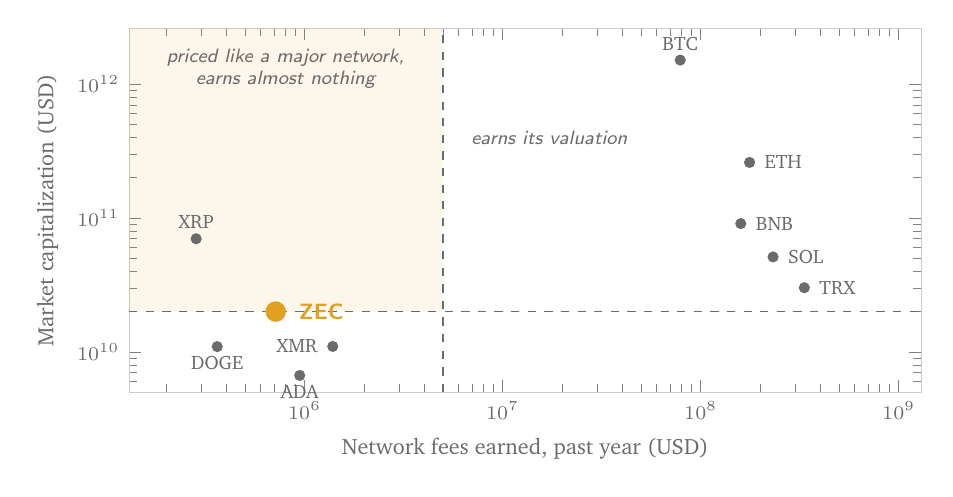
\begin{tikzpicture}
\begin{axis}[
  width=0.96\linewidth, height=6.2cm,
  xmode=log, ymode=log,
  xmin=1.3e5, xmax=1.3e9, ymin=5e9, ymax=2.6e12,
  axis line style={draw=rulegray},
  xlabel={\footnotesize Network fees earned, past year (USD)},
  ylabel={\footnotesize Market capitalization (USD)},
  xlabel style={font=\footnotesize\color{mid}}, ylabel style={font=\footnotesize\color{mid}},
  tick label style={font=\scriptsize\color{mid}},
  clip=false,
]
\fill[zecgold,opacity=0.09] (axis cs:1.3e5,2e10) rectangle (axis cs:5e6,2.6e12);
\draw[dashed,draw=mid,line width=0.5pt] (axis cs:5e6,5e9) -- (axis cs:5e6,2.6e12);
\draw[dashed,draw=mid,line width=0.5pt] (axis cs:1.3e5,2e10) -- (axis cs:1.3e9,2e10);
\node[font=\scriptsize\sffamily\itshape,text=mid,align=center] at (axis cs:8e5,1.3e12) {priced like a major network,\\earns almost nothing};
\node[font=\scriptsize\sffamily\itshape,text=mid,anchor=west] at (axis cs:6.2e6,4e11) {earns its valuation};
\addplot[only marks,mark=*,mark size=1.8pt,draw=mid,fill=mid] coordinates {
 (78867169,1509454765402)(176603888,259847421784)(159390509,90742383993)
 (232034579,51154819765)(333782586,30124728512)(1386327,10971866799)
 (361943,10941146556)(944239,6663993692)(283228,69897197724)};
\node[font=\scriptsize,text=mid,anchor=south] at (axis cs:78867169,1509454765402) {BTC};
\node[font=\scriptsize,text=mid,anchor=west] at (axis cs:176603888,259847421784) {\;ETH};
\node[font=\scriptsize,text=mid,anchor=west] at (axis cs:159390509,90742383993) {\;BNB};
\node[font=\scriptsize,text=mid,anchor=west] at (axis cs:232034579,51154819765) {\;SOL};
\node[font=\scriptsize,text=mid,anchor=west] at (axis cs:333782586,30124728512) {\;TRX};
\node[font=\scriptsize,text=mid,anchor=east] at (axis cs:1386327,10971866799) {XMR\;};
\node[font=\scriptsize,text=mid,anchor=north] at (axis cs:361943,10941146556) {DOGE};
\node[font=\scriptsize,text=mid,anchor=north] at (axis cs:944239,6663993692) {ADA};
\node[font=\scriptsize,text=mid,anchor=south] at (axis cs:283228,69897197724) {XRP};
\addplot[only marks,mark=*,mark size=3.5pt,draw=zecgold,fill=zecgold] coordinates {(714314,19976953357)};
\node[font=\footnotesize\sffamily\bfseries,text=zecgold,anchor=west] at (axis cs:714314,19976953357) {\;\;ZEC};
\end{axis}
\end{tikzpicture}
\figcap{Figure 2.}{Every current top ten asset, market cap against trailing year fees, log scales. Zcash is the only asset marketed on network usage that sits in the top left. One more tell: its annualized volatility is about 132\%, two to three times Bitcoin, Ethereum, or Monero. Top ten assets do not move like that. Source: CoinGecko, DefiLlama, Artemis.}
\end{center}

\subsection{It is not sound money either}
The bull reply is that Zcash is not a business but money, a private Bitcoin, so fees are the wrong lens. Fine. Then it has to clear the bar that money clears, and it does not. In 2026 researchers disclosed a counterfeiting flaw in the Orchard shielded pool that had been live for about four years and could have minted unlimited coins that nobody could see. The network patched it, but because every transaction is hidden, not even the developers can prove it was never used. Zcash fell about 64\% around that disclosure. For an asset whose entire pitch is sound, verifiable money, a stretch of years where the supply could not be trusted is disqualifying, and it is the opposite of Bitcoin, whose supply anyone can audit in seconds. The rest of the soundness story is no better. The founding team at the Electric Coin Company resigned in January, and the price fell about 14\% that week. Issuance still runs near 3.3\% a year, and a fifth of every block goes to a developer fund rather than to holders. Security is bought with inflation, not usage: over the last 90 days, 99.8\% of what miners earned was newly printed supply and 0.2\% was fees. And the privacy is optional, so under a third of the supply is ever shielded. Higher inflation, recently unauditable, run by a fund after its founders walked out, with privacy most holders never use. That is not a smaller Bitcoin.

\subsection{Catalysts, and the bull case we have to beat}
To be fair to the other side, the bull case is not empty. Arthur Hayes has said Zcash could reach ten to twenty percent of Bitcoin's value, and Multicoin and Paradigm both bought in. The pitch is that privacy becomes scarce as artificial intelligence makes everything else traceable, and that Zcash is the cleanest public way to own it. I take that seriously. The trouble is that the catalysts meant to carry it are either already in the price or already turning. The spot fund that was the big new buyer has flipped to outflows. The Winklevoss treasury built to absorb supply trades below the value of its own coins, so the market will no longer pay it a premium to keep buying. And the scheduled events ahead cut against holders: the developer fund that takes a fifth of issuance is up for debate, miners keep selling new supply, and NU7 now routes most of the few fees that exist away from security. There is no catalyst left that is both large and unpriced. What remains is a story carried by a crowded, levered long.

\textbf{Risks to the short, stated plainly.}
\begin{itemize}
  \item Momentum and the squeeze. Zcash is in a strong uptrend and short covering has repeatedly fed it. We size small, lean on the measurable gap, and respect a move to \$2,000.
  \item A spot fund that reaccelerates, renewed treasury buying, or a fresh wave of the privacy narrative would extend the mania. We weight this as a real adverse case.
  \item Usage is genuinely rising, and a regulatory overhang in some places could cut either way. We treat regulation as a secondary risk, not the thesis.
\end{itemize}

% ======================= 3. INVESTMENT PROPOSAL =======================
\section{Investment Proposal}

Position: short Zcash. Entry near \$1,170. Horizon: 6 to 12 months. The trade resolves as a price built on a story reverts toward the fundamentals and comparables that support it. The targets are not guesses, they come from the one honest comparable. Zcash has about 17 million coins. A base case near \$650 puts its market cap close to Monero's, around \$11 billion, which is where a privacy leader that earns less than Monero and shields less than Monero should sit. A deeper case near \$450 takes it below Monero, near \$8 billion, on its optional privacy and governance risk. We weight the outcomes 20\% deeper, 45\% base, and 35\% a squeeze to \$2,000, which still leaves a modest positive expected value on a high variance trade.

\subsection{Valuation on the metrics that matter}
We value Zcash through three lenses, and they converge. First, revenue, the metric this panel built: Zcash trades near twenty eight thousand times its network fees, where productive chains sit between about ninety and fifteen hundred, so it is among the most expensive large assets in crypto. Second, comparables: Monero earns nearly twice the fees and clears several times the real private payments for a little over half the market cap, so Zcash carries a privacy premium of about two times that its usage does not justify. Third, the holder base: the marginal buyers are a fund that is now selling and a treasury underwater on the market's own view, while miners add about 3\% of new supply a year and sell it. Fundamentals, comparables, and flows all point the same way.

\subsection{Why this is the trade}
We also set a line we would be wrong at. If network revenue rose by an order of magnitude, or if the shielded share of supply passed a clear majority, the thesis would be broken and we would cover. Neither is close today. We are not shorting Zcash because it went up. We are shorting a gap we can measure, between a top ten price and a network that earns almost nothing and a kind of money that is weaker than the one it imitates. The reflexive buyers that built the premium, a levered futures bid and a treasury already underwater on the market's view, are the most likely to accelerate the reversal.

% ======================= 4. CONCLUSION =======================
\section{Conclusion}

Zcash is a genuinely improved network wrapped in a valuation its fundamentals do not support. The usage is rising and the narrative has never been louder, but none of that underwrites a \$20 billion price on an asset that earns about \$712,000 of fees a year, shields under a third of its supply, trades at nearly twice the market cap of the privacy coin that does more real payment, and could not prove its own supply for four years. Priced as a network, it is one of the most expensive in crypto. Priced as money, it is weaker than Bitcoin on every axis that makes money sound. The market is paying for a story, financial privacy in the age of AI, as if it were adoption. On the metrics that define value accrual, Zcash has not earned its place in the top ten, and the bid that carried it there is already turning.

\textbf{Recommendation: short Zcash over a 6 to 12 month horizon. Base target \$650, about 44\% downside. Deeper target \$450. Acknowledged squeeze risk toward \$2,000. The narrative is loud. The revenue is not, and the money is not sound. That gap is the trade.}

\vspace{10pt}
{\color{zecgold}\hrule height 0.9pt}
\vspace{8pt}
\noindent
\begin{minipage}[t]{0.31\linewidth}\centering{\sffamily\bfseries\fontsize{18}{20}\selectfont +44\%}\\[3pt]{\scriptsize\sffamily\color{mid}\MakeUppercase{Base, ZEC \$650}}\end{minipage}\hfill
\begin{minipage}[t]{0.31\linewidth}\centering{\sffamily\bfseries\fontsize{18}{20}\selectfont +62\%}\\[3pt]{\scriptsize\sffamily\color{mid}\MakeUppercase{Deeper, ZEC \$450}}\end{minipage}\hfill
\begin{minipage}[t]{0.31\linewidth}\centering{\sffamily\bfseries\fontsize{18}{20}\selectfont (71\%)}\\[3pt]{\scriptsize\sffamily\color{mid}\MakeUppercase{Squeeze, ZEC \$2,000}}\end{minipage}
\vspace{8pt}
{\color{zecgold}\hrule height 0.9pt}

% ======================= APPENDIX =======================
\clearpage
\section*{Appendix \quad {\normalsize\mdseries\color{mid} Six exhibits behind the short}}
\vspace{2pt}

\noindent
\begin{minipage}[t]{0.47\linewidth}
\exlabel{1 \quad What you pay per dollar of fees}
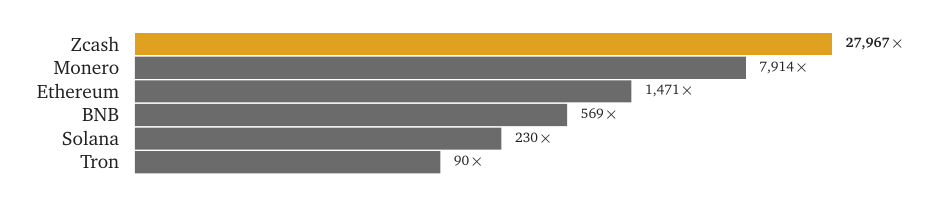
\begin{tikzpicture}
\begin{axis}[
  width=\linewidth, height=3.5cm, xbar, bar width=8pt, bar shift=0pt,
  xmin=0, xmax=5.3, axis x line=none, axis y line=left,
  y axis line style={draw=none}, ytick style={draw=none},
  symbolic y coords={Tron,Solana,BNB,Ethereum,Monero,Zcash},
  ytick={Tron,Solana,BNB,Ethereum,Monero,Zcash},
  yticklabel style={font=\scriptsize\color{ink}}, enlarge y limits=0.14, clip=false,
]
\addplot[draw=none,fill=mid] coordinates {(1.95,Tron)(2.34,Solana)(2.76,BNB)(3.17,Ethereum)(3.90,Monero)};
\addplot[draw=none,fill=zecgold] coordinates {(4.45,Zcash)};
\node[right,font=\tiny,text=ink] at (axis cs:1.95,Tron) {\;90$\times$};
\node[right,font=\tiny,text=ink] at (axis cs:2.34,Solana) {\;230$\times$};
\node[right,font=\tiny,text=ink] at (axis cs:2.76,BNB) {\;569$\times$};
\node[right,font=\tiny,text=ink] at (axis cs:3.17,Ethereum) {\;1,471$\times$};
\node[right,font=\tiny,text=ink] at (axis cs:3.90,Monero) {\;7,914$\times$};
\node[right,font=\tiny\bfseries,text=ink] at (axis cs:4.45,Zcash) {\;27,967$\times$};
\end{axis}
\end{tikzpicture}
\excap{Market cap divided by trailing year fees, log scale. Source: DefiLlama, CoinGecko.}
\end{minipage}\hfill
\begin{minipage}[t]{0.47\linewidth}
\exlabel{2 \quad It trades like a small cap}
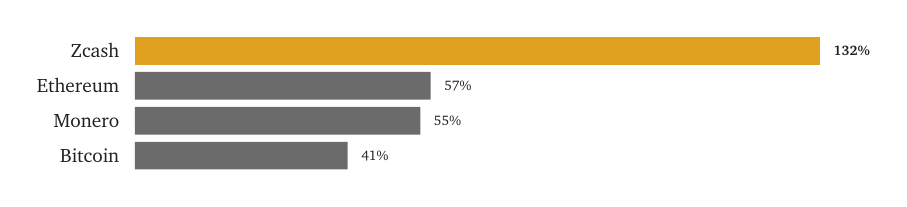
\begin{tikzpicture}
\begin{axis}[
  width=\linewidth, height=3.5cm, xbar, bar width=10pt, bar shift=0pt,
  xmin=0, xmax=160, axis x line=none, axis y line=left,
  y axis line style={draw=none}, ytick style={draw=none},
  symbolic y coords={Bitcoin,Monero,Ethereum,Zcash},
  ytick={Bitcoin,Monero,Ethereum,Zcash},
  yticklabel style={font=\scriptsize\color{ink}}, enlarge y limits=0.22, clip=false,
]
\addplot[draw=none,fill=mid] coordinates {(41,Bitcoin)(55,Monero)(57,Ethereum)};
\addplot[draw=none,fill=zecgold] coordinates {(132,Zcash)};
\node[right,font=\tiny,text=ink] at (axis cs:41,Bitcoin) {\;41\%};
\node[right,font=\tiny,text=ink] at (axis cs:55,Monero) {\;55\%};
\node[right,font=\tiny,text=ink] at (axis cs:57,Ethereum) {\;57\%};
\node[right,font=\tiny\bfseries,text=ink] at (axis cs:132,Zcash) {\;132\%};
\end{axis}
\end{tikzpicture}
\excap{Annualized price volatility, 90 day. Source: Artemis, our own calc from daily prices.}
\end{minipage}

\vspace{12pt}
\noindent
\begin{minipage}[t]{0.47\linewidth}
\exlabel{3 \quad Half the cap, far less usage}
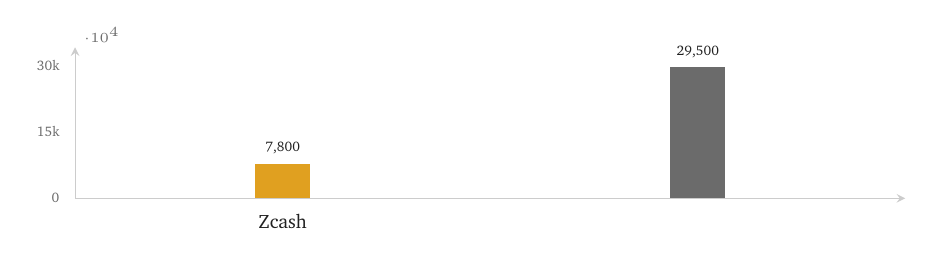
\begin{tikzpicture}
\begin{axis}[
  width=\linewidth, height=3.5cm, ybar, bar width=20pt, bar shift=0pt,
  ymin=0, ymax=34000, axis x line=bottom, axis y line=left,
  x axis line style={draw=rulegray}, y axis line style={draw=rulegray},
  symbolic x coords={Zcash,Monero}, xtick=data, tick style={draw=none},
  xticklabel style={font=\scriptsize\color{ink}},
  ytick={0,15000,30000}, yticklabels={0,15k,30k},
  yticklabel style={font=\tiny\color{mid}}, enlarge x limits=0.5, clip=false,
]
\addplot[draw=none,fill=zecgold] coordinates {(Zcash,7800)};
\addplot[draw=none,fill=mid] coordinates {(Monero,29500)};
\node[font=\tiny,text=ink,anchor=south] at (axis cs:Zcash,7800) {7,800};
\node[font=\tiny,text=ink,anchor=south] at (axis cs:Monero,29500) {29,500};
\end{axis}
\end{tikzpicture}
\excap{Daily transactions, November 2026. Monero, at half the cap, does about 4x the volume, all of it private. Source: CoinMetrics.}
\end{minipage}\hfill
\begin{minipage}[t]{0.47\linewidth}
\exlabel{4 \quad Security bought with inflation}
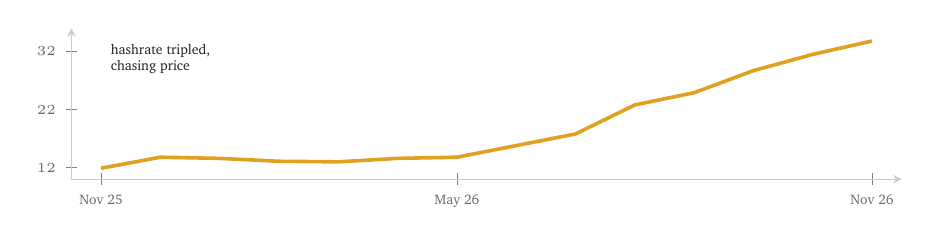
\begin{tikzpicture}
\begin{axis}[
  width=\linewidth, height=3.5cm,
  ymin=10, ymax=36, xmin=0.5, xmax=14.5,
  axis x line=bottom, axis y line=left,
  x axis line style={draw=rulegray}, y axis line style={draw=rulegray},
  xtick={1,7,14}, xticklabels={Nov 25,May 26,Nov 26},
  xticklabel style={font=\tiny\color{mid}},
  ytick={12,22,32}, yticklabel style={font=\tiny\color{mid}}, clip=false,
]
\addplot[zecgold,line width=1.3pt] coordinates {(1,11.9)(2,13.8)(3,13.6)(4,13.1)(5,13.0)(6,13.6)(7,13.8)(8,15.8)(9,17.8)(10,22.8)(11,24.9)(12,28.7)(13,31.5)(14,33.8)};
\node[font=\tiny,text=ink,anchor=north west,align=left] at (axis cs:1,35) {hashrate tripled,\\chasing price};
\end{axis}
\end{tikzpicture}
\excap{Hashrate (gigasol per second). Over 90 days, 99.8\% of miner pay was new issuance, 0.2\% fees. Source: zecmetrics, The DeFi Report.}
\end{minipage}

\vspace{12pt}
\noindent
\begin{minipage}[t]{0.47\linewidth}
\exlabel{5 \quad A four year bug, a 64\% crash}
\vspace{1pt}
\colorbox{goldtint}{\begin{minipage}{0.95\linewidth}\vspace{2pt}
{\footnotesize\color{ink}
A counterfeiting flaw in the Orchard pool sat live for \textbf{about four years}. It could have minted \textbf{unlimited} coins, and because privacy hides everything, \textbf{nobody can prove it was never used}. Around the disclosure Zcash fell \textbf{64\%} (\$685 to \$247) with about \textbf{\$118M} of liquidations.}
\vspace{2pt}\end{minipage}}
\excap{Source: Allium onchain research, CoinDesk.}
\end{minipage}\hfill
\begin{minipage}[t]{0.47\linewidth}
\exlabel{6 \quad The reflexive bid is cracking}
\vspace{1pt}
\colorbox{goldtint}{\begin{minipage}{0.95\linewidth}\vspace{2pt}
{\footnotesize\color{ink}
The Cypherpunk treasury trades about \textbf{18\% below} the value of its own Zcash. The Grayscale fund hit \$1B of assets on only about \textbf{\$306M} of real inflows, then lost a \textbf{\$93.6M} week. Open interest is about \textbf{13\%} of market cap and the tape is \textbf{14x} more futures than spot.}
\vspace{2pt}\end{minipage}}
\excap{Source: DefiLlama, SEC filings, CoinGlass.}
\end{minipage}

\vspace{14pt}
{\footnotesize\color{mid} Data note. Market caps, prices, and supply are as of early November 2026, from CoinGecko cross checked against the Blockworks market series. Network fees for every chain are trailing year figures pulled from the DefiLlama API, one consistent methodology, so Zcash is compared like for like. Zcash has no out of protocol tips or extractable value, so fees are its entire network revenue, which the Blockworks Zcash Token Holder Report puts at about \$204,000 for the third quarter. Volatility is annualized from daily prices and cross checked against Artemis. Every figure in this report is reproducible from a small set of free data scripts. Zcash versus Monero transactions from CoinMetrics. The Orchard disclosure and the June 2026 crash are documented by Allium, the competition's other research tool.}

% ======================= REFERENCES =======================
\clearpage
\section*{References}

\begin{enumerate}[leftmargin=1.5em,itemsep=2pt,topsep=2pt]
  \item Blockworks Research. Zcash Token Holder Report, third quarter 2026, and the real economic value framework.
  \item DefiLlama. Trailing year network fees for Zcash, Monero, Ethereum, Solana, Tron, and peers, November 2026.
  \item CoinGecko. Market capitalization and price for Zcash, Monero, and the top ten assets, November 2026.
  \item CoinMetrics. Zcash and Monero transactions, active addresses, and price history.
  \item Artemis. Zcash 30 and 90 day annualized volatility, November 2026.
  \item Allium. A Four Year Bug, a 64 Percent Crash, and a Question Nobody Can Close, onchain research, 2026.
  \item Chun Wang, F2Pool. Public commentary describing the Zcash rally as a narrative bid.
  \item Grayscale. Zcash, Financial Privacy in the Age of AI, and the spot Zcash fund flows.
  \item The DeFi Report and zecmetrics. Zcash hashrate, miner revenue mix, and issuance.
  \item Electric Coin Company. Founding team departures and governance, January 2026; Cypherpunk Technologies treasury disclosures; CoinGlass futures data.
\end{enumerate}

\end{document}
